\chapter{Principal Component Analysis COMING SOON}
\label{ch-pca}


%https://en.wikipedia.org/wiki/Principal_component_analysis

%
%https://online.stat.psu.edu/stat508/lessons/Lesson07

This chapter is based on Ref.\cite{wiki-pca}.

{\bf Principal Component Analysis} (PCA)

PCA is one of several possible ways of doing 
{\bf Dimensionality Reduction} (See Chapter \ref{ch-dim-reduc})

\begin{itemize}


\item{\bf Notation}

$X=[x_1, x_2, \ldots, x_\calf]\in \RR^{N\times \calf}$ {\bf Initial dataset} to be dimensionality reduced. Assume $X$ has {\bf zero mean} throughout. If $X$ doesn't have zero mean initially, 
replace $X_{\s, i}$ by 
$X_{\s, i}-\frac{1}{N}\sum_\s X_{\s, i} $


$Y=[y_1, y_2, \ldots, y_\calf]\in \RR^{N\times \calf}$. The $y_i$ for $i=1,2, \ldots, \calf$ are called the {\bf principal components} (PCs).

$u\in \RR^{N\times 1}$

$U= [u_1, u_2, \ldots u_{N}]
\in\RR^{N \times N}$, $UU^T =U^TU =1$ ($U$ orthogonal)
 
$\Lam= \left[\begin{array}{c}
\Lam_D\\
0^{(N-\calf)\times \calf}
\end{array}\right]\in\RR^{N\times \calf}$, $\Lam_D=diag(\lam_1, \lam_2, \ldots, \lam_{\calf})$

$v\in \RR^{\calf\times 1}$

$W= [w_1, w_2, \ldots w_{\calf}]\in\RR^{\calf\times \calf}$, $WW^T=W^TW=1$
($W$ orthogonal)

{\bf Singular Value Decomposition} (SVD)
\beq X = U\Lam W^T
\eeq

\item {\bf Covariance Matrix}
\beqa
X^T X &=& W \Lam^T U^T U \Lam W^T
\\
&=& W \Lam^T \Lam W^T
\\
&=& W \Lam_D^2 W^T
\eeqa

\beq
[X^T X]_{i,j} = X_{\s, i} X_{\s, j}=W_{i, r}\lam^2_rW_{r, j}
\eeq
We will refer to $\lam_i^2$ and to $w_i=[W_{i, r}]_{r=1}^\calf$
as the {\bf principal value} (PV)
and the {\bf principal axis} (PA) 
of $X$.

\beqa
Y &=& XW\\
&=& U\Lam W^T W
\\\
&=&
U \Lam 
\eeqa
$Y= U\Lam$ is called the Polar Decomposition of $Y$

\beq
Y_{\s, i} = X_{\s, j}W_{j,i}=U_{\s, i}\lam_{i}
\eeq


\beqa
[Y^T Y]_{i,j}&=&Y_{\s, i} Y_{\s, j}
\\&=& 
U_{\s, i}\lam_{i} U_{\s, j}\lam_{j}
\\&=&
\lam_{i}^2\delta_{i,j}
\eeqa

\beq
Y_{\s, i} = X_{\s, j}W_{j,i}=U_{\s, i}\lam_{i}
\eeq



\item{\bf PCA as solution to Maximization problem}
\beqa
W_{\cdot,1}&=&
\argmax_{W_{\cdot,1}: \sum_j W_{j,1}^2=1}\sum_\s (Y_{\s, 1})^2 
\\
&=& \argmax_{W_{\cdot,1}: \sum_j W_{j,1}^2=1}\sum_\s (X_{\s, j}W_{j,1})^2
\\
&=& \argmax_{W_{\cdot,1}}\sum_\s
\frac{(X_{\s, j}W_{j,1})^2}{W_{j,1}W_{j,1}}
\eeqa


\beq
X_{\s, i}^\Phi = X_{\s, i} -\sum_{k=1}^{\Phi-1}
\underbrace{X_{\s, a}W_{a,k}W^T_{k,i}}_{
\Delta X^k_{\s, i}}
\label{eq-X-super-f}
\eeq
If we multiple Eq.(\ref{eq-X-super-f}) by $ W_{i, j}$,
and sum over $i$, we get

\beqa
Y_{\s, j}^\Phi &=& Y_{\s, j} -\sum_{k=1}^{\Phi-1}
\underbrace{X_{\s, a}W_{a,k}}_{Y_{\s, k}}\delta_{k, j}
\\
&=& Y_{\s, j}
-Y_{\s, j}\indi(j\leq\Phi-1)
\label{eq-Y-super-f}
\eeqa
See Fig.\ref{fig-XY-super-f}
for a pictorial
representation of Eqs.\ref{eq-X-super-f}
and \ref{eq-Y-super-f}.


\begin{figure}[!h]
$$
\begin{array}{ccc}
\xymatrix@R=5pc@C=4pc{
&\ar[l]_{\Delta X^1}
&\ar[l]_{\Delta X^2}
&\ar[l]_{\Delta X^3}
\\
\ar[u]|{X^1=X}
\ar[ur]|{X^2}
\ar[urr]|{X^3}
\ar[urrr]|{X^4}
}
&\text{ times $W$ =}&
\xymatrix@R=5pc@C=4pc{
&\ar[l]_{\Delta Y^1}
&\ar[l]_{\Delta Y^2}
&\ar[l]_{\Delta Y^3}
\\
\ar[u]|{Y^1=Y}
\ar[ur]|{Y^2}
\ar[urr]|{Y^3}
\ar[urrr]|{Y^4}
}
\end{array}
$$
\caption{Pictorial representation of Eqs.\ref{eq-X-super-f}and
\ref{eq-Y-super-f}.
This figure is not accurate in the sense that the vectors
$\Delta X^1, \Delta X^2, \Delta X^3$ are in reality not coplanar. Also,
$X^\Phi$ and $Y^\Phi$ both tend to zero as $\Phi\rarrow \calf$.}
\label{fig-XY-super-f}
\end{figure}


\beqa
W_{\cdot,\Phi}&=&
 \argmax_{W_{\cdot,\Phi}: \sum_j W_{j,\Phi}^2=1}\sum_\s (X^\Phi_{\s, j}W_{j,\Phi})^2
 \\
 &=& \argmax_{W_{\cdot,\Phi}}\sum_\s
 \frac{(X^\Phi_{\s, j}W_{j,\Phi})^2}{W_{j,\Phi}W_{j,\Phi}}
 \eeqa
 
\item {\bf Truncation}
\beq
Y_{\s, i\leq \Phi} = X_{\s, j}W_{j,i\leq \Phi}=U_{\s, i}\lam_{i\leq \Phi}
\eeq


\beq
Y_{\leq \Phi} = XW_{\leq \Phi} = U\Lam_{\leq \Phi}
\eeq

\beq
Y-Y_{\leq \Phi} = U(\Lam - \Lam_{\leq \Phi})
\eeq


\beqa
Error &=& 
\tr\left[(X-X_{\leq \Phi})^T(X-X_{\leq \Phi})\right]
\\
&=& \tr\left[(X-X_{\leq \Phi})^T W W^T(X-X_{\leq \Phi})\right]
\\
&=& \tr\left[(Y-Y_{\leq \Phi})^T(Y-Y_{\leq \Phi})\right]
\\
&=&
\tr\left[(\Lam - \Lam_{\leq \Phi})^2\right]
\\
&=&
\sum_{i=\Phi+1}^\calf \lam_i
\eeqa

\item {\bf PCA calculation}

Note that $Y=XW$, where $X$ is the initial dataset and $W$ is the matrix that diagonalizes the covariance matrix $X^T X$. Hence, calculating $Y$
does not require calculating the SVD of $X$ (in particular, it does not require calculating $U$). 

PCA calculation via Covariance Matrix
\begin{enumerate}
\item Subtract mean from initial dataset $X$
\item Diagonalize covariance matrix 

\beq
X^TX=W^T \Lam^2 W=\lam^2_j w_j w_j^T
\eeq
\item Order eigenvalues in diagonal of $\Lam^2$ and corresponding rows of $W$ so that eigenvalues $\lam^2_i$ are in decreasing order.
\item Calculate $Y= XW$
\end{enumerate}

Iterative calculation of PCA

$r^{(0)}_j\in \RR^{\calf \times 1}$ random column vector. $s^{(0)}_j=0^{\calf \times 1}$ zero column vector .


\beq
x_j = [X_{\s, j}]_{\s=1}^N
\;\; \text{(column vector)}
\eeq

\beq
s_{j}^{(a+1)} = s_j^{(a)} + x_j  [x^T_jr_j^{(a)}] 
\eeq


\beq
\lam_j^{(a)} = r^{(a)T}_j s_j^{(a)}
\eeq

\beq
r_{j}^{(a+1)} =\frac{s_j^{(a+1)}}{\norm{s_j^{(a+1)}}}
\eeq
If we calculate $s_j^{(a)}$ for large $a$, and for $j=1, 2, \ldots \calf$, we get an approximation of
$X^T X r^{(a)}\rarrow w_1$ and 
$r^{(a)T}X^T X r^{(a)}\rarrow \lam_1$ where
$(\lam_1, w_1)$ are the first PV and PA of $X$.

Additional PCs are obtained by {\bf deflation}. 
For example, the second PC is obtained by 
replacing $X$ by $X -\lam_1 w_1 w_1^T$ and following the same algorithm that we used to
calculate the 1st PC of $X$.

\item {\bf Plots}
 
 
 Suppose the unit column vectors $w_1,
 w_2\in\RR^{\calf\times 1}$
 are the first two PA, and $\lam_1^2, \lam_2^2$ are the corresponding PVs.
 
 {\bf PC scores} are $(X_{\s, i}w_{i, 1},
 X_{\s, i}w_{i, 2})$ for all data points $\s$.
 
 
 Let $e_f\in \RR^{\calf\times 1}$ 
 be a one hot vector with 1 at position $f$.
 
 
 If $e_{g, f}w_{g, f' }= e_f\cdot w_{f'}$,
 then $(e_f\cdot w_1, e_f\cdot w_2)$ are the {\bf loadings} (i.e., weights) for feature $f$.
 
 Fig.\ref{fig-scree} is a plot of the
 PVs $\lam_i^2$ versus $i$. Such a plot is 
 called a {\bf scree plot}.
 
 Fig.\ref{fig-scores-loadings-biplot}
 shows three types of plots: a {\bf PC scores plot}, a {\bf loadings plot}, and a biplot. A {\bf biplot} is a superposition
 of the PC scores plot and the loadings plot.
 \end{itemize}
 
\begin{figure}[h!]
\centering
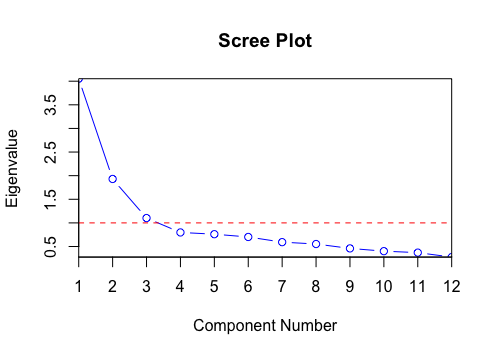
\includegraphics[width=5in]
{pca/scree.png}
\caption{Scree plot. (from Wikipedia entry "Scree plot")
For a geologist, a scree is the edge of a cliff. It looks just like the blue 
curve in this figure, like a decaying exponential.}
\label{fig-scree}
\end{figure}

\begin{figure}[h!]
\centering
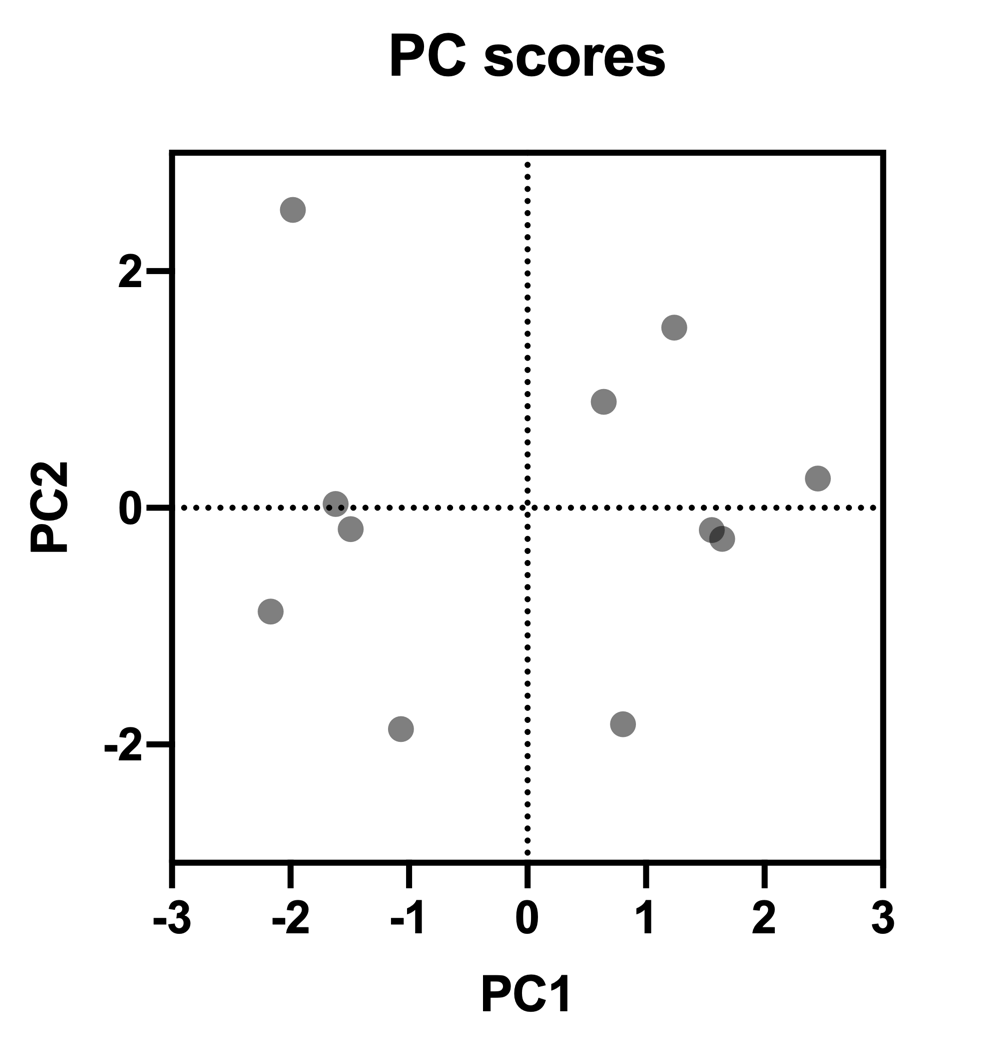
\includegraphics[width=2.5in]
{pca/pc-scores.png}
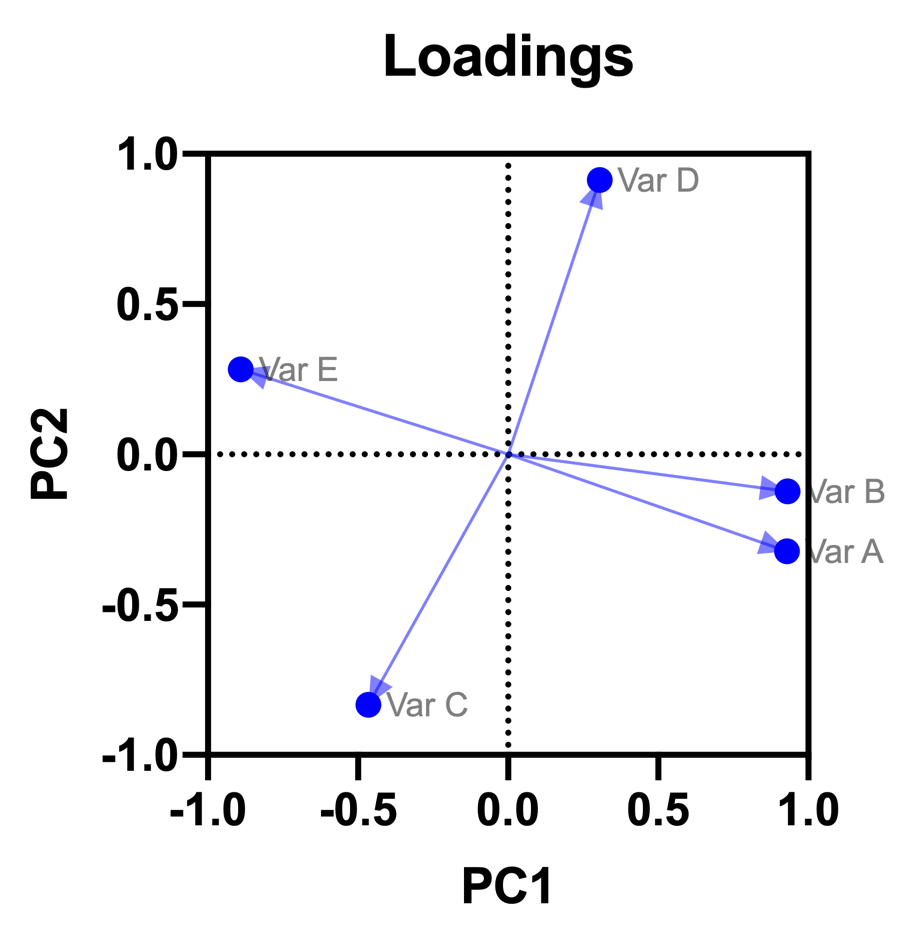
\includegraphics[width=2.5in]
{pca/loadings.png}
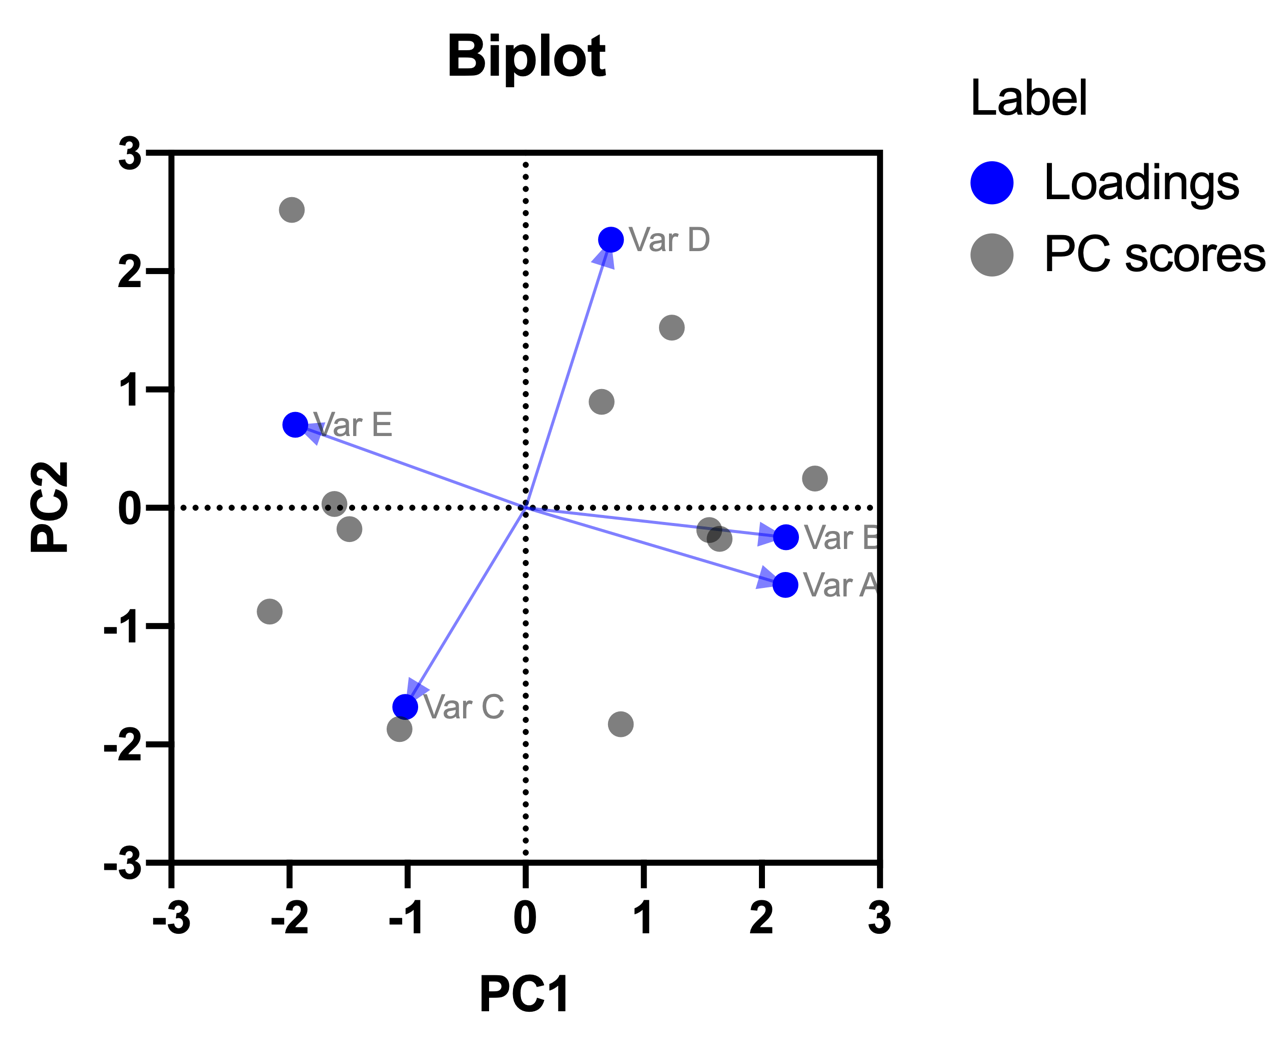
\includegraphics[width=5in]
{pca/biplot.png}

\caption{PC scores plot, loadings plot, and biplot. (from the documentation for the Prism software made by graphpad.com)}
\label{fig-scores-loadings-biplot}
\end{figure}

